\documentclass[review, authoryear]{elsarticle}   	% use "amsart" instead of "article" for AMSLaTeX format
\usepackage{geometry}                		% See geometry.pdf to learn the layout options. There are lots.
\usepackage{pdflscape}
\usepackage{graphicx}				% Use pdf, png, jpg, or eps§ with pdflatex; use eps in DVI mode
\usepackage{amssymb, amsmath}
\usepackage{topcapt}
%\usepackage[round]{natbib}
\usepackage{booktabs}
\usepackage{subscript}
\usepackage{textcomp}
\usepackage{marginnote}


%%
\usepackage[colorinlistoftodos, textwidth=4cm, shadow]{todonotes}
\DeclareRobustCommand{\Carlos}{\todo[author=Carlos, inline, color=blue!40, size=\small]}
\DeclareRobustCommand{\Jhoa}{\todo[author=Jhoa, inline, color=yellow!40, size=\small]}
%%
\usepackage{lineno,hyperref}
\modulolinenumbers[5]

\journal{Ocean \& Coastal Management}

%% `Elsevier LaTeX' style
\bibliographystyle{elsarticle-harv}

\begin{document}

\begin{frontmatter}

\title{Carbon stocks in aboveground biomass for Colombian mangroves with associated uncertainties}
\author[MPI,CYB]{Jhoanata M. Bolivar}
\author[TU,CYB]{Victor H. Gutierrez-Velez}
\author[MPI,CYB]{Carlos A. Sierra}
\address[MPI]{Max Planck Institute for Biogeochemistry, Hans-Kn\"oll-Str. 10, 07745 Jena, Germany}
\address[CYB]{Research Center on Ecosystems and Global Change Carbono \& Bosques, Medell\'in, Colombia}
\address[TU]{Department of Geography and Urban Studies, Temple University, Philadelphia, PA 19122, USA}

%\date{}							% Activate to display a given date or no date


\begin{abstract}
Decision-making process, as well as the implementation of future climate change mitigation strategies for mangrove ecosystems, need the availability of reliable base information and tools to estimate the carbon stocks at regional and national levels. We estimated carbon (C) stocks in aboveground biomass (AGB) for mangroves in the Caribbean and Pacific coasts of Colombia. Using available data on AGB density and mangrove area for the whole country (excluding islands) and each coast independently, we estimated a national carbon stock in AGB for Colombian mangroves as 14.95 $\pm$ 2.72 TgC (mean $\pm$ SE), with 2.20 $\pm$ 0.86 TgC in the Caribbean coast and 9.61 $\pm$ 2.78 TgC in the Pacific coast. Uncertainty for total carbon in AGB in Colombian mangroves, reported as SE/mean in percentage, was 18\% at the national level, 39\% in the Caribbean coast, and 29\% in the Pacific coast. This uncertainty was more influenced by uncertainties associated with the estimation of mangrove area for the Caribbean coast, while for the Pacific coast it was more influenced by the uncertainties associated with AGB density. This difference is the result of a contrasting availability of AGB density data for both coasts.  Comparison between observed AGB density data and predictions from large-scale models showed that these models underestimate AGB density for Colombian mangroves. We reparameterized these models with our data, but found poor goodness-of-fit statistics for these model structures. We propose therefore three new statistical models to predict AGB density in Colombian mangroves based on climatic and vegetation data. In all cases, the best models included the enhanced vegetation index (EVI) and the mean temperature of driest quarter (BIO9). 
\end{abstract}

\begin{keyword}
Blue carbon \sep uncertainty analysis \sep aboveground biomass \sep EVI \sep national carbon inventory
\end{keyword}

\end{frontmatter}

%Highlights
%

\linenumbers

\section{Introduction}

Efforts to reduce tropical deforestation have traditionally focused on terrestrial environments; however, recent studies investigating the contribution of coastal ecosystems to mitigate climate change through carbon storage suggest that these ecosystems can rival their terrestrial counterparts \citep{Donato2011}. Coastal vegetated ecosystems, in particular mangroves, salt marshes, and seagrasses conform Earth's `blue carbon' sinks \citep{Herr2012}. They comprise only  0.05\% of the plant biomass on land, but store a comparable amount of carbon per year, and thus rank among the most important carbon sinks on the planet \citep{Nellemann2009}. 

%Given their capacity as carbon sinks, coupled with other ecosystem services they provide and regulate, the management of these coastal ecosystems has strong potential to be a transformational tool in sustainable livelihoods, climate resilience, and a valuable part of global natural carbon management \citep{Boucher2014}. Despite their importance, they are disappearing or becoming degraded as result of economic development in coastal areas \citep{Pendleton2012}.

Among these blue carbon ecosystems, mangroves have an enormous capacity for carbon storage \citep{Nellemann2009, Donato2011, Adame2013}, and may pose serious risks for greenhouse gas (GHG) emissions due to land use change in coastal areas \citep{WorldBank2010}. Unfortunately, there is a large data gap at regional scales about carbon storage in mangroves \citep{Donato2011}, so their inclusion in national climate change mitigation strategies is still limited. This data gap hinders the possibility of mangrove ecosystems to participate in current climate change mitigation schemes such as Reducing Emissions from Deforestation and Forest Degradation (REDD+) as well as Nationally Appropriate Mitigation Actions (NAMAs)\citep{Alongi2011, Herr2012, Murray2012, Boucher2014}. %To face this barrier, it is necessary to build awareness in the climate change policy community about the strength of the capacity of carbon storage in mangroves, through enhance the scientific and technical basis for financing of mangrove management activities \citep{Herr2012}.  

Participation in climate change mitigation schemes will require countries to produce accurate estimates of their forest carbon stocks with their change over time through robust Measurement, Reporting and Verification (MRV) programs \citep{Cohen2013968}. To achieve the required quality level, it is important \emph{to assess the quality of measurements taken in the field, data compilation and analysis data in order to generate error estimates and improve future measurements} \citep{Maniatis2010}. Furthermore, the success of blue carbon projects depends to a large degree on the reliability of the scientific information used for their implementation (Alongi 2011, Maniatis and Mollicone, 2010). In this sense, it is necessary to quantify and report uncertainties in estimates of carbon stocks for these ecosystems \citep{Kauffman2012, Alongi2011} as well as the main sources that contribute to the uncertainty in the carbon stock estimates. 

%In this sense, taking into account the existing uncertainties in the biophysical dynamics of "blue carbon" resources \citep{Kauffman2012, Alongi2011}, the identification of potential sources of uncertainty and the implementation of measures to reduce it could help to providing robuster estimates of carbon stock for different pools of forest, including above ground biomass (AGB).

Two sources of information are necessary for the estimation of temporal changes in GHG emissions or GHG emission reductions in forests: emission factors (i.e. carbon stocks changes) and activity data (i.e. changes in areas under a specific land use). The Intergovernmental Panel on Climate Change \citep{IPCC2003, IPCC2006} highlights the necessity to provide estimations for these two sources of information with a level of uncertainty as low as possible (according with the capacity of the country), reporting mean estimates along their 95\% confidence limits. In this respect, it is necessary to provide uncertainty estimates for both carbon stocks and area in determining the baseline for climate change mitigation projects \citep{Maniatis2010}. 

%In that way, taking into account that AGB/carbon stocks data as well as area information are the base line to estimate those changes, low uncertainties associated to that information is equally relevant \citep{Maniatis2010}. 

Estimates of carbon stocks changes can be obtained using different approaches. The \citet{IPCC2003, IPCC2006} has categorized these approaches in three different levels: Tier 1, Tier 2, and Tier 3; with increasing accuracy and complexity in MRV from Tier 1 to Tier 3 \citep{Maniatis2010}. 
%In this sense, the information about Emission Factors as well as Activity Data, increase the accuracy from Tier 1 to Tier 3, as well as increases in complexity of monitoring and analysis \citep{Maniatis2010}.
For the estimation of forest carbon stocks, particularly in aboveground biomass (AGB), information about mangrove cover area, forest-plot inventory data as well as statistical models are combined to obtain carbon stock estimates for particular regions. These three different sources of information contain uncertainties that must be propagated to the final estimate.  For plot inventory data, uncertainties are generally associated with sampling errors, the use of allometric models, and other systematic errors \citep{Chave2005, Sierra2007}. For mangrove cover area, uncertainty is related with the ability to detect and delineate accurately areas that correspond to mangroves. Detection of cover area can be done with field-surveys, aerial photographs, or satellite products, and these areas should correspond to the areas or the ecological characteristics where biomass estimates are available.  Lastly, a model must be used to scale-up plot-level data to landscape and regional levels. Model predictions also contain uncertainty related to model structure and parameter values \citep{IPCC2006}. To propagate uncertainty from these different sources, one can either propagate analytically standard deviations or standard errors using known formulas, or use Monte Carlo methods \citep{Chave2005, Sierra2007, IPCC2006}.

%Uncertainties associated to these components could be associated to sampling errors and systematic errors. To estimate carbon stocks at national level, general models which include parameters available for all mangrove areas in the country like those associated with climatic variability and location are more useful. In this sense, models uncertainty can be derived from two main components: uncertainty in the structure of the model and uncertainty in the parameter values \citep{IPCC2006}. 

In Colombia, estimates of carbon stocks in mangroves are available only for a few locations. Data for these sites was produced for research projects or to establish the baseline of carbon stocks for the future implementation of pilot REDD+ at the project level \citep{Yepes2016, Malaga2015}. Despite the importance of these efforts, C stock estimates for mangroves are not articulated with the mitigation strategy being designed at the national level. For instance,  a recent estimation of national carbon stocks \citep{Phillips2011} did not include mangroves as an independent category, underestimating the capacity of the country to mitigate climate through terrestrial C sinks.

%Aware of this situation, \citet{Phillips2011} proposed that current estimates of carbon stocks at the national level for Colombia are revised to identify additional criteria for classification of those ecosystems that were not well represented (e.g., seasonality, soil types, flooding, etc.) and obtain a proper estimation of carbon stocks and their spatial variability. At the same time, these authors point out that current estimations have high levels of uncertainty, in contrast to the Intergovernmental Panel on Climate Change (IPCC) guidelines that recommend low levels of uncertainty in estimations of carbon stocks (near to 10\%) for biomass in natural forests.

Given that national estimates of carbon stocks are relevant inputs for decision-making and implementation of future climate change mitigation strategies, it is necessary to adjust carbon stocks estimates for mangrove ecosystems reducing current uncertainties. To achieve this goal, it is important to identify sources of uncertainty at regional (different coastlines) and at national scales, and in this way, to prioritize actions to reduce it. Additionally, the development of tools such as AGB models at the national scale could help to identify the relevance of different mangrove areas as carbon sinks, including predictive variables that account for significant levels of spatial variability \citep{Ewel1998, Kristensen2008}. %Both efforts could help with the integration of mangroves in the current national mitigation schemes due to the capacity building which could help to overcome the current barriers for their inclusion.

The main objectives of this study were: (i) to estimate the current uncertainty in the estimation of the national carbon stock in AGB for mangrove ecosystems in Colombia, identifying sources of uncertainty and proposing possible ways to reduce it; and (ii) to develop a statistical model to predict carbon stocks at the national level. We present estimates not only for the entire country, but also for mangroves in each coast, Caribbean and Pacific. 

%Carbon stock estimations and associated uncertainties are presented not only for the whole country but also for mangroves at each coast (Caribbean and Pacific). We made this separation because we believe it is possible to find differences about sources of uncertainties between coasts, taking into account differentiated efforts of sampling and characterisation of mangrove ecosystems, availability of data and absence of standard methodologies for both area and AGB estimation, with a marked effort in Caribbean mangroves. By the other hand, we hope to find that global models as well as national model developed in the framework of this study could not be enough to explain all variability of our data due to the existence of significant differences in physical characteristics in mangrove habitats at continental, regional and local scales \citep{Ewel1998} which affect the conditions of carbon transformation and transport through the ecosystem \citep{Kristensen2008}.



\section{Methods}
\subsection{Data sources}
We used carbon data from two different sources: (i) scientific articles and/or technical reports from studies developed in mangrove areas located in the Caribbean and Pacific coast of Colombia, in which aboveground biomass (AGB) was quantified and; (ii) data from two inventories of carbon stocks in Cispat\'{a} bay (Colombian Caribbean coast) and M\'{a}laga bay (Colombian Pacific coast) \citep{Yepes2016, Malaga2015}. For the first type of data, we selected only studies that included coordinates or specific location names that can be easily geolocated \citep{INVEMAR2007, Lema2007, DelaPena2010, Blanco2012}. The main difference between both data types is the scale of the information. The first data type report average AGB per location, while the second data type reports estimates per plot covering the same region  (22 permanent plots of 500 m\textsuperscript2 in Cispat\'{a} bay  and 10 in M\'{a}laga bay). AGB data sources used to develop the predictive models are provided in the supplementary material.  

The number of sources used reflects the scarce availability of public information in Colombia regarding biomass studies in mangrove ecosystems. Only those studies published with open access, or referenced in the Information System for the Management of Mangroves in Colombia (SIGMA) were used. Additionally, despite that more biomass inventories have been conducted in the Colombian mangroves, only those provided by INVEMAR could be accessed. The differences in terms of scale of the two sources of information, as well as the impossibility to include the different mangrove types along the two coasts, result in limitations in terms of the scope of our results. Nevertheless, considering the goal of the study, this first approach is a relevant step to identify the necessities of sampling in order to reduce the current uncertainties associated to the carbon stock estimation at national and/or regional level.

For our upscaling strategy, we used bioclimatic data and remote sensing products on the state of vegetation. 
Bioclimatic data were extracted from the WorldClim Bioclim \citep{Hijmans2005} 30 arc-second data set (http://www.worldclim.org/bioclim). WorldClim is a set of global climate layers (gridded climate data) with a spatial resolution of about 1 km\textsuperscript2. The bioclimate variables are derived from the monthly temperature and rainfall values.

Data on vegetation condition consisted of the Enhanced Vegetation Index values extracted from the MOD13Q1 MODIS Vegetation Indices Product. The product represents 16-day composites at 232 m spatial resolution. We selected EVI over the Normalized Difference Vegetation Index, also included in the MOD13Q1 product because it offers better sensitivity to forest canopy variations, specially in areas with high biomass \citep{Huete2002}. %\marginpar{Huete, A., K. Didan, T. Miura, E. P. Rodriguez, X. Gao, and L. G. Ferreira. 2002. Overview of the radiometric and biophysical performance of the MODIS vegetation indices. Remote Sensing of Environment 83:195-213.}. 
EVI values were retrieved from the online data pool, courtesy of the NASA Land Processes Distributed Active Archive Center (LP DAAC) \citep{MODIS2015} (https://lpdaac.usgs.gov/data\_access/data\_pool). The MOD13 product comes with three levels of pixel reliability. For our purpose, we extracted all pixel values with good and marginal reliability for the years 2011 through 2013. These years cover the time range in which most of the carbon plots considered for the analysis were established. We included the marginal reliability pixels because the number of good quality pixels is not engough to cover the whole study area, given their high cloud cover throughout the year, specially in the Pacific coast. After pixels values were extracted, we excluded pixels that had a reflectance in the blue band higher than 10 percent because these pixels are tipically associated to clouds. We also removed unreliable pixels based on abrupt drop or spikes in the data time series \citep{Gutierrez2013}. %\marginpar{Gutiérrez-Vélez, V. H., and R. DeFries. 2013. Annual multi-resolution detection of land cover conversion to oil palm in the Peruvian Amazon. Remote Sensing of Environment 129:154-167}. 
Finally, we derived  the mean EVI per pixel within the study area.

% Requires the booktabs if the memoir class is not being used
\begin{table}[htbp]
   \centering
   \topcaption{Bioclimatic variables used for modeling (see www.worldclim.org/bioclim)} % requires the topcapt package
   \begin{tabular}{p{2cm}p{7cm}p{3cm}} % Column formatting, @{} suppresses leading/trailing space
      \toprule
       Variable   & Name & Type\\
      \midrule
      BIO1         & Annual mean temperature (\textcelsius)  & Average and seasonalities \\
      BIO4         & Temperature seasonality: S.D. of monthly mean temperature  &  Average and seasonalities \\
      BIO12       & Annual precipitation (mm)  & Average and seasonalities \\
      BIO15       & Precipitation seasonality: CV of monthly precipitation  & Average and seasonalities \\
      BIO9         & Mean Temperature of Driest Quarter (\textcelsius)&  Extremes\\
      BIO10       & Mean Temperature of warmest quarter (\textcelsius)&  Extremes\\
      BIO11       & Mean Temperature of coldest quarter (\textcelsius)&  Extremes\\ 
      BIO16       & Precipitation of the wettest quarter (mm)&  Extremes\\
      BIO17       & Precipitation of the driest quarter (mm)&  Extremes\\
      \bottomrule
   \end{tabular}
   %\caption{Bioclimatic variables used for modeling (see www.worldclim.org/bioclim)}
   \label{tab:booktabs}
\end{table}

%\begin{figure}[htbp]
%   \centering
%   \includegraphics{Figures/map.pdf} % requires the graphicx package
%\caption{Spatial distribution of mangroves in Colombia (green dots) and location of study sites with AGB density information (red stars)%.}
%   \label{fig:map}
%\end{figure}
%
Furthermore, information about mangrove cover area comes from two different sources: global estimations \citep{FAO2007, Giri2011, Giri2011dataset, CONL:CONL12060} and national estimations compiled by the Colombian institute for ocean and coastal research \citep{INVEMAR2014} and derived from particular estimations made by the different environmental authorities with jurisdiction in mangrove areas along the country. Those mangrove areas were estimated under different methodological approaches.

\subsection{Estimation of national carbon stocks from available data and associated uncertainties}
We pooled the available AGB density data by coast and for the entire country and calculated averages, standard deviations, and standard errors at each level. To report results in units of C, we used a conversion factor of 0.5 as recommended by other authors \citep{MacDicken1997, Clark2001, Fearnside2004, Chave2005, Aragao2009}. We also calculated averages from the available data on mangrove areas for each coast and the entire country. Based on the obtained averages and standard errors for each variable, we calculated national and regional carbon stocks using a Monte Carlo procedure in which we sampled 1000 random deviates from a normal distribution with mean equal to the average from the available data and standard deviation from their standard errors. We multiplied both sets of 1000 random deviates (AGB density $\times$ mangrove area) to obtain a set of 1000 random numbers with mean equal to the expected C stock for each region and standard deviation for the mean according to the Central Limit Theorem \citep[see also][]{Sierra2007}. Therefore, we report uncertainties for the mean AGB, mean mangrove area, and mean C stock.

To report uncertainties, we use the coefficient of variation CV calculated as the ratio SE to the mean for sample data, and as SD to mean for Monte-Carlo-simulated variables.

To identify whether the uncertainty in the regional and national C stocks are mostly contributed by uncertainties in AGB density or mangrove area and the efforts that must be made to reduce it, we developed a sensitivity analysis based on different levels of uncertainty for each contributing variable. We assumed values of uncertainty of 0\%, 5\%, 10\%, 15\%, 20\%, 30\%, 50\% and 100\% (as CV in percentage) for each variable and calculated the uncertainty in the regional or national C stock for all possible combinations.

%We used AGB data available for some mangroves areas located in La Guajira, Magdalena, C\'{or}doba and Antioquia departments (Caribbean coast) and Valle del Cauca department (Pacific coast) to estimate the average carbon stock  in mangroves for the country as well as per coast (Caribbean and Pacific). We considered a conversion factor from biomass to carbon of 0.50, as is proposed by several authors \citep{MacDicken1997, Clark2001, Fearnside2004, Chave2005, Aragao2009}.  Likewise, we estimated the total carbon stock in mangroves for each coast and for the whole country using the area calculated for Colombian mangroves for \citet{INVEMAR2014}, the estimation derived from Global Mangrove Forests Distribution, 2000 \citep{Giri2011dataset, Giri2011} and also the Colombian mangrove cover area related by \citet{CONL:CONL12060} and \citet{FAO2007} (OJO PORQUE ME QUEDA LA CITA ASI). 

%We included in the total carbon estimation the uncertainty (in terms of standard error (SE)) associated with the Area and AGB, taking into account the differences between the area reported for the different sources of information and the values of biomass per hectare estimated for each one of the localities included. Likewise, we  did an sensitivity analysis of  the Coefficient of Variation (CV) of the total AGB under different levels of uncertainty (0\%, 5\%, 10\%, 15\%, 20\%, 30\%, 50\% and 100\%) to establish the effect of those uncertainties leves on the determination of Carbon stocks in Colombian mangroves.

\subsection{Predictive models}
We used available models published in the scientific literature to predict AGB for the locations where we have data and evaluated the possibility of using these models for our regional and national estimations. We evaluated the latitude-based model developed by \citet{Twilley1992} and the climate-based model developed by \citet{CONL:CONL12060}. Given that we obtained very poor performance of these models in predicting our observations (see Results section), we developed our own set of predictive models for AGB with regression analysis. 

We evaluated different functional response models to explain the AGB at each location \emph{i}:

\begin{align}
AGB_{i} &= a+bX_{i}+e_{i}, \\
%\end{equation}
%\begin{equation}
\frac{1}{AGB_{i}} &= a+b\frac{1}{X_{i}}+e_{i}, \\
%\end{equation}
%\begin{equation}
\log{AGB_{i}} &= a+bX_{i}+e_{i}, \\
%\end{equation} 
%\begin{equation}
\log{AGB_{i}} &= a+b\log{X_{i}}+e_{i}, \\
%\end{equation} 
%\begin{equation}
\log{AGB_{i}} &= a+b\frac{1}{X_{i}}+e_{i}, 
\end{align} 
where $X_i$ represents the value of a predictive variable at the location $i$, with an error $e_i$, and coefficients $a$ and $b$. As predictive variables, we evaluated latitud, the Enhanced Vegetation Index (EVI) from MODIS \citep{MODIS2015}, bioclimatic variables form the WorldClim dataset \citep{Hijmans2005}, and possible combinations among all variables. We evaluated in total 48 models. For parameter estimation, we used ordinary least squares using function {\tt lm} in R.

The latitude data were used to calculate distance from the equator, which has been previously related to mangrove productivity \citep{Twilley1992, Saenger1993, Komiyama2008128, Wang2013539, Alongi2014}.  Working with the assumption that mangrove biomass will be affected by temperature and precipitation \citep{Komiyama2008128, CONL:CONL12060}, average and extreme bioclimatic variables proposed by \citet{CONL:CONL12060} were included as well as precipitation and temperature associated to the driest quarter (Table \ref{tab:booktabs}). 

Model performance was assessed using the adjusted coefficient of determination (R\textsubscript{a}\textsuperscript{2}), which informs about in-sampling predictive power, and the Akaike information criterion with a correction for finite sample sizes (AICc), indicating model generalizability as it relates to model simplicity \citep{1748-9326-9-10-104013}.

We used the R package AICcmodavg \citep{Mazerolle:2015aa} to compare candidate models that showed the best predictive power and simplicity through a ``model selection table" based on the AIC. This table assigns to each model a weight, which could be interpreted as the probability of an  \emph{i} model to be the best of the evaluated group of models. %Likewise, classification of models according with their weight is possible to get with this package. In this sense, 
Candidate models can be classified in four categories according to these weights: ``substantial weight models", ``some weight models", ``little weight models" and ``no weight models". We selected models classified in the ``substantial weight"  and ``some weight" groups as models to be used in biomass predictions.  

To determine the influence of environmental local variability on AGB, we also fitted multilevel models through maximum likelihood estimation using the R package lme4 \citep{Bates:2015aa}. We assumed our data as classified into two subgroups, site and Coastal Environmental Units (CEU). The first subgroup refers to the specific location of the sites, while the CUE refers to an environmental classification of coastal zones in Colombia \citep{LopezRodriguez2013}. We estimated the initially proposed models including separately each subgroup, but also the interaction between both. The predictive power of the model was analyzed using the Deviance statistic (D\textsuperscript{2}\%), which measures the percentage of the variability explained by the model. 

\subsection {AGB estimation using the predictive models}
We estimated model-average predictions of AGB based on the candidate models classified as ``substantial weight models'' category, according to the results of the ``model selection table'' describe in the above section. Model-average predictions were carried out weighting each model by its AIC weight. We scaled-up AGB predictions using data on EVI and bioclimatic variables for the known mangrove areas in both coasts. 

%EVI data base used for the estimation was got from \Jhoa {ACA ES NECESARIO TENER CLARA LA FUENTE DE INFORMACIÓN DE VICTOR}. For the same points associated with EVI data, we obtained the WorldClim bioclimatic variables BIO9 and BI016.


\section{Results}

\subsection{National carbon stock estimation from available data and associated uncertainties}
\subsubsection{Mangrove areas}
Published approaches for the estimation of mangrove areas at the country level vary from one study to another. The methodological spectrum goes from studies using global approaches like those reported by  \citet{Giri2011dataset, Giri2011} and  \citet{CONL:CONL12060} using remote sensing products,  to studies focused on regional surveys using land verification  \citep{FAO2007}, and a compilation individual estimates developed at a local scale under different methodologies \citet{INVEMAR2014} (Table \ref{tab:areaMethods}). 

We found that mean mangrove area for the Pacific coast was around four times larger than mean mangrove area for the Caribbean coast. We obtained larger uncertainties in terms of area for the Caribbean than for the Pacific coast. In terms of the total mangrove area of the country, the uncertainty was bigger for area than for AGB density (Table \ref{tab:means}).

% Requires the booktabs if the memoir class is not being used
\begin{landscape}
\begin{table}[htbp]
   \centering
   \topcaption{Mangrove areas in Colombia as reported in different sources of information and with different methodological approaches} % requires the topcapt package
   \begin{tabular}{p{2cm}p{1cm}p{2cm}p{2cm}p{2cm}p{10cm}} % Column formatting, @{} suppresses leading/trailing space
      \toprule
       Source  & Year & Caribbean coast (ha) & Pacific coast (ha) & Total country (ha) & Methodological Approach\\
      \midrule
      \citet{INVEMAR2014}         & 2004-2013  & 69 894.02 & 239 239.20 & 300 133.22 & Areas calculated from individual estimates by administrative units (departments) with mangrove cover in Colombia. Methodological approach used for each specific case is not reported in the document. Date of estimation is variable between departments.\\
      \citet{Giri2011dataset, Giri2011}          & 2000  &  47 064.78 &  165 563.6 & 212 628.4 & Compilation of the extent of mangroves forests from the Global Land Survey and the Landsat archive with hybrid supervised and unsupervised digital image classification techniques. The data are available at 30-m spatial resolution. Area estimated under the assumption that each coordinate in the country represent a raster pixel of 900 m\textsuperscript2.\\
      \citet{Giri2011dataset, Giri2011}          & 2000  & 13 846.07 & 144 882.74 & 158 728.21 & Compilation of the extent of mangroves forests from the Global Land Survey and the Landsat archive with hybrid supervised and unsupervised digital image classification techniques. The data are available at 30-m spatial resolution. Area estimated using ArcGis version 10.2.2 Software.\\
     \citet{FAO2007}      & 1997  & & & 371 250 &  Caribbean: interpretation of satellite images. Pacific: aerial photographs, radar and satellite images. Land verification, specifying mangrove areas with help of  1:100 000 scale maps. \\
      \citet{CONL:CONL12060}       & 1999 - 2003& & &410 152 & Spatial information extracted from mangrove map developed by \citet{Spalding2010}. Landsat images, using a variety of image-processing techniques and with considerable expert review. \\
            \bottomrule
   \end{tabular}
   %\caption{Bioclimatic variables used for modeling (see www.worldclim.org/bioclim)}
   \label{tab:areaMethods}
\end{table}
\end{landscape}

\subsubsection{Aboveground biomass density}
For the case of AGB density, estimates from the literature correspond to different spatial scales, thus, for the case of mangroves in C\'ordoba department in the Caribbean coast and Valle del Cauca department in the Pacific coast, available AGB density was linked with individual plots while for the rest of the areas the available data correspond to estimation for wider locations (e.g. type of forest, physiographic location, etc.) (see supplementary information). 

When AGB density for both coasts are compared, the average values do not differ significantly between each other. In terms of uncertainty, larger values of the CV were observed for AGB density in the Pacific coast than in the Caribbean coast. 

% Requires the booktabs if the memoir class is not being used
\begin{table}[htbp]
   \centering
   \topcaption{mean, standard deviation (SD), standard error (SE) and coefficient of variation (CV) for Area and AGB density in Colombian mangroves.} % requires the topcapt package
   \begin{tabular}{p{1.5cm}p{1.8cm}p{1.8cm}p{1.8cm}p{1.0cm}p{1.0cm}p{1.0cm}p{1.0cm}p{1.0cm}} % Column formatting, @{} suppresses leading/trailing space
      \toprule
      
       Region & \multicolumn{4}{c}{Area (ha)} & \multicolumn{4}{c}{AGB density (Mg/ha)}\\
      &mean&SD&SE&CV&mean&SD&SE&CV\\
            \midrule
      Caribbean&43 601.62&28 184.01&16 272.04&0.37&102.20&58.42&9.74&0.09\\
      Pacific&183 228.50&49 596.60&28 634.61&0.16&105.58&83.13&26.29&0.25\\
      Colombia&290 578.40&105 306.40 &47 094.44&0.16&102.93&63.55&9.37&0.09\\
            \bottomrule
   \end{tabular}
   \label{tab:means}
\end{table}


\subsubsection{Regional and national AGB carbon stocks}
Given the different sources of information used for mangrove area published at the whole country and every coast independently (Table \ref{tab:areaMethods}), the sum of total carbon in AGB estimated for both coasts does not match exactly to the value reported for the whole country (Table \ref{tab:meansTotal}). However, both estimates overlap in their uncertainty ranges. 

Total carbon in AGB showed larger values in Pacific mangroves (9.61 $\pm$ 2.78 TgC) (mean $\pm$ SE) than in Caribbean mangroves (2.20 $\pm$ 0.86 TgC). This result is highly influenced by mangrove area, because if the comparison is made in terms of the same area unit (hectare), values of carbon density between both coasts do not show significant differences (Figure 1 %\ref{fig:Csotck}). 

%\begin{figure}
%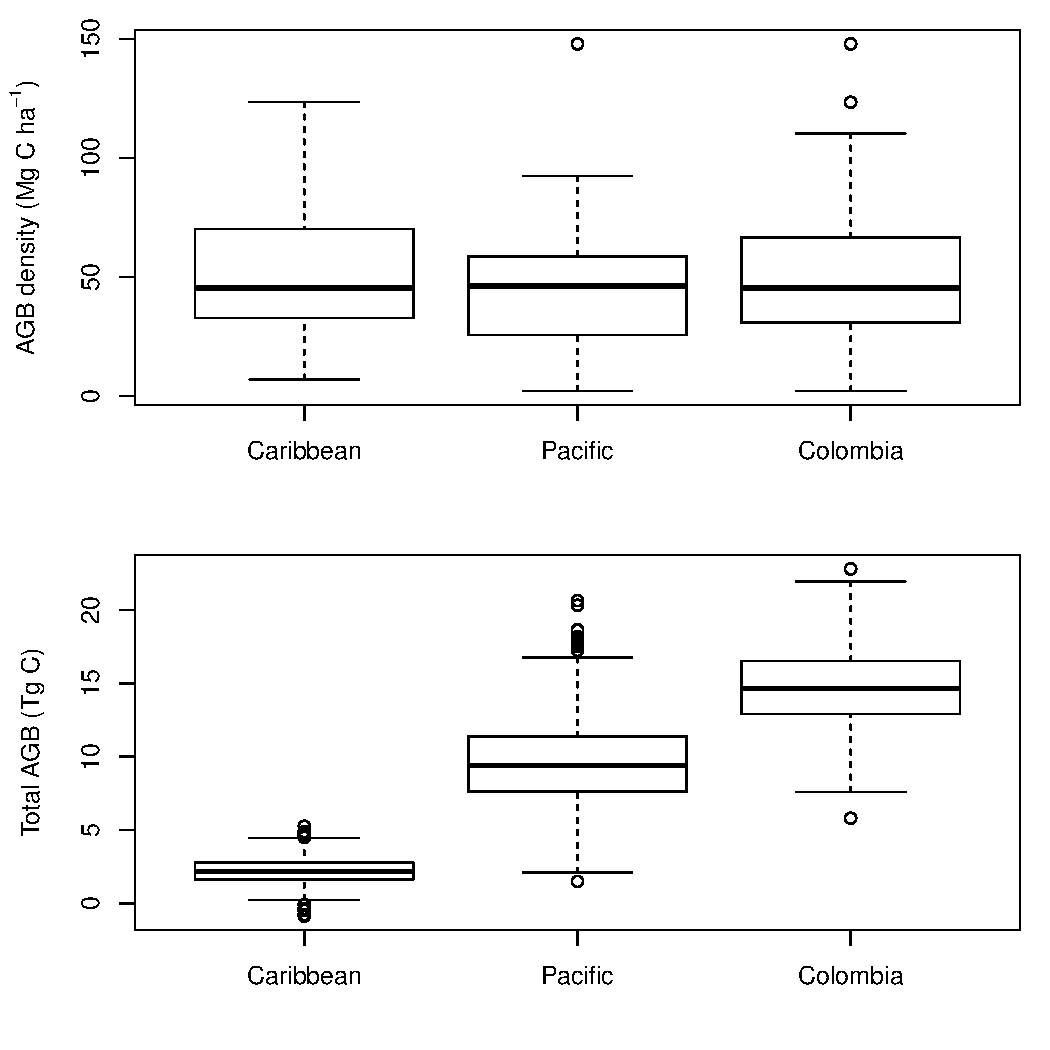
\includegraphics[%scale=0.4
%width=\textwidth
%]{Figures/Cdensity_and_TotalCstock.pdf} 
%\caption{
Figure 1. Aboveground biomass (AGB) density (Mg C ha$^{-1}$) and total carbon stock in AGB for Colombian mangroves (Tg C). 
%}
%\label{fig:Csotck}
%\end{figure}

The ratio between the SE and the mean total carbon stock showed larger uncertainty for Caribbean mangroves than for Pacific mangroves. For the case of the total area of mangroves in Colombia, the uncertainty was lower than for every coast analyzed independently (Table \ref{tab:meansTotal}). Connecting this result with findings related to CV estimated for mangrove areas and AGB density independently (Table \ref{tab:means}), it is possible to conclude that uncertainties of total carbon stock in AGB for mangroves located in the Caribbean coast are more influenced by uncertainties associated with mangrove area estimation. Contrastingly, for mangroves located in the Pacific coast this uncertainty in total AGB carbon stock is more influenced by uncertainties in AGB density. At the country level, total uncertainty is more influenced by current uncertainty in mangrove area. 

% Requires the booktabs if the memoir class is not being used
\begin{table}[htbp]
   \centering
   \topcaption{Mean of total C in AGB (Tg), standard error (SE), coefficient of variation (CV) and quantiles 10\% and 90\% for Colombian mangroves.} % requires the topcapt package
   \begin{tabular}{p{3.0cm}p{2.0cm}p{2.0cm}p{2.0cm}p{2.0cm}p{2.0cm}} % Column formatting, @{} suppresses leading/trailing space
      \toprule
       Region & mean & SE & CV & \multicolumn{2}{c}{quantiles}\\
      \midrule
      &&&&10\%&90\%\\
      Caribbean&2.20&0.86&0.39&1.14&3.31\\
      Pacific&9.61&2.78&0.29&6.26&13.79\\
      Colombia&14.95&2.72&0.18&11.51&18.52\\
            \bottomrule
   \end{tabular}
   \label{tab:meansTotal}
\end{table}

%NOTA: COMO EL CARBONO TOTAL POR COSTA Y PARA EL PAIS FUE ESTIMADO TENIENDO EN CUENTA QUE PARA EL TOTAL DEL PAIS EL PROMEDIO INVOLUCRO MAS DATOS, NUNCA VA A COINCIDIR LA SUMA DE LAS DOS COSTAS CON EL TOTAL REPORTADO.

\subsubsection{Sensitivity of total uncertainty to uncertainty in mangrove area and AGB density}

%The sensitivity analysis of the uncertainty in total AGB associated to interactions between AGB density and mangrove area shows a similar tendency for both coasts as well as at the country level. In all cases, CV increased with increasing uncertainty for both components. An increase in a 10\% of uncertainty level leads to an increase of CV in $\approx$ 0.10, either when the analysis is made given priority to AGB or area (Tables \ref{tab:sensCaribbean}, \ref{tab:sensPacific} and \ref{tab:sensCol}). CV values for different levels of uncertainty are similar for all three cases (Caribbean, Pacific and Colombia), the only notable change is registered at maximum level of uncertainty (interaction of uncertainty level for AGB 100\% with uncertainty level for Area 100\%), in this case, CV for Caribbean mangroves (1.84) is bigger than CV for Pacific coast (1.51) and data of all country (1.65). 

The sensitivity analysis allowed us to determine the effort necessary to reduce uncertainty in AGB density and/or mangrove area and achieve a desirable level of uncertainty for total AGB carbon stock estimations. Under different levels of uncertainty, we projected different levels of CV of total AGB carbon stocks for both coast as well as for the whole country (Tables \ref{tab:sensCaribbean}, \ref{tab:sensPacific} and \ref{tab:sensCol}). 

% Requires the booktabs if the memoir class is not being used
\begin{table}[htbp]
   \centering
   \topcaption{Uncertainty (CV) in total AGB C stock associated to interactions between uncertainty in AGB density and mangrove area for the Caribbean coast} % requires the topcapt package
   \begin{tabular}{p{2.0cm}p{1.0cm}p{1.0cm}p{1.0cm}p{1.0cm}p{1.0cm}p{1.0cm}p{1.0cm}p{1.0cm}p{1.0cm}} % Column formatting, @{} suppresses leading/trailing space
      \toprule
        &&\multicolumn{8}{c}{Levels of uncertainty mangrove area}\\      
      &&0\%&5\%&10\%&15\%&20\%&30\%&50\%&100\%\\
            \midrule 
Levels of uncertainty AGB&0\%&0.00&0.05&0.10&0.15&0.19&0.31&0.48&0.99\\ 
      &5\%&0.05&0.07&0.11&0.16&0.20&0.31&0.48&1.00\\
     &10\%&0.10&0.11&0.14&0.18&0.22&0.32&0.49&1.00\\
      &15\%&0.16&0.17&0.19&0.22&0.25&0.35&0.51&1.02 \\
      &20\%&0.19&0.20&0.22&0.24&0.27&0.37&0.53&1.02\\
     &30\%&0.30&0.30&0.32&0.33&0.35&0.42&0.59&1.05\\
 &50\%&0.48&0.49&0.50&0.51&0.52&0.58&0.71&1.20\\
     &100\%&0.95&0.95&0.95&0.97&0.98&1.09&1.16&1.59\\
               \bottomrule
   \end{tabular}
   \label{tab:sensCaribbean}
\end{table}

% Requires the booktabs if the memoir class is not being used
\begin{table}[htbp]
   \centering
   \topcaption{Uncertainty (CV) in total AGB C stock associated to interactions between uncertainty in AGB density and mangrove area for the Pacific coast} % requires the topcapt package
   \begin{tabular}{p{2.0cm}p{1.0cm}p{1.0cm}p{1.0cm}p{1.0cm}p{1.0cm}p{1.0cm}p{1.0cm}p{1.0cm}p{1.0cm}} % Column formatting, @{} suppresses leading/trailing space
      \toprule
        &&\multicolumn{8}{c}{Levels of uncertainty mangrove area}\\      
      &&0\%&5\%&10\%&15\%&20\%&30\%&50\%&100\%\\
            \midrule 
Levels of uncertainty AGB&0\%&0.00&0.05&0.10&0.15&0.20&0.31&0.51&1.03\\ 
      &5\%&0.05&0.07&0.11&0.16&0.20&0.31&0.51&1.03\\
     &10\%&0.10&0.11&0.14&0.18&0.22&0.32&0.32&1.00\\
      &15\%&0.15&0.16&0.18&0.22&0.25&0.35&0.53&1.06\\
      &20\%&0.25&0.21&0.23&0.24&0.28&0.37&0.55&1.06\\
     &30\%&0.31&0.31&0.33&0.34&0.36&0.44&0.62&1.12\\
 &50\%&0.50&0.50&0.51&0.52&0.56&0.62&0.75&1.31\\
     &100\%&1.00&1.00&1.01&1.02&1.03&1.09&1.21&1.84\\
               \bottomrule
   \end{tabular}
   \label{tab:sensPacific}
\end{table}


% Requires the booktabs if the memoir class is not being used
\begin{table}[htbp]
   \centering
   \topcaption{Uncertainty (CV) in total AGB C stock associated to interactions between uncertainty in AGB density and mangrove area for Colombian mangroves} % requires the topcapt package
   \begin{tabular}{p{2.0cm}p{1.0cm}p{1.0cm}p{1.0cm}p{1.0cm}p{1.0cm}p{1.0cm}p{1.0cm}p{1.0cm}p{1.0cm}} % Column formatting, @{} suppresses leading/trailing space
      \toprule
        &&\multicolumn{8}{c}{Levels of uncertainty mangrove area}\\      
      &&0\%&5\%&10\%&15\%&20\%&30\%&50\%&100\%\\
            \midrule 
Levels of uncertainty AGB&0\%&0.00&0.05&0.10&0.15&0.20&0.30&0.47&1.02\\ 
      &5\%&0.05&0.07&0.11&0.16&0.20&0.31&0.48&1.02\\
     &10\%&0.10&0.11&0.14&0.18&0.22&0.32&0.49&1.03\\
      &15\%&0.15&0.16&0.18&0.21&0.26&0.35&0.50&1.04\\
      &20\%&0.24&0.20&0.22&0.24&0.28&0.37&0.51&1.07\\
     &30\%&0.31&0.31&0.32&0.35&0.37&0.43&0.57&1.10\\
 &50\%&0.51&0.51&0.48&0.53&0.55&0.61&0.74&1.28\\
     &100\%&1.00&1.00&1.02&1.02&1.04&1.08&1.20&1.75\\
                    \bottomrule
   \end{tabular}
   \label{tab:sensCol}
\end{table}

Reducing current total AGB carbon stock uncertainty to 10\% can be achieved under different combinations of reductions in AGB density uncertainty and mangrove area uncertainty. Achieving  this level of uncertainty implies one of two options: (i) reduce uncertainty in area to 5\% and maintain the current uncertainty in AGB density (9\%) (in the case of the Caribbean coast and the whole country) or reducing it at 10\% (in the case of Pacific coast); or (ii) reduce uncertainty in mangrove area to 10\% and simultaneously reduce uncertainty in AGB density to 5\%. 

Both alternatives to achieve 10\% uncertainty level for total AGB C stock imply different efforts according with the current uncertainties associated to every input data (AGB density and mangrove area) for each coast. For instance, reduction in terms of mangrove area implies more effort for the Caribbean mangroves (current level of uncertainty 37\%), while for the Pacific more effort is needed to reduce  current uncertainty associated with AGB density (25\%). 

To achieve a 10\% uncertainty in AGB density for the Pacific coast, it would be necessary to establish at least 47 new sampling units, and a 5\% uncertainty may not be possible to achieve with less than 200 sampling units (Figure 2%\ref{fig:samplingEffort}). For the Caribbean coast the situation is less critical; it is possible to achieve a 5\% uncertainty in AGB density by adding 73 additional sampling units. Combined for the entire country, 81 additional sampling units are required to achieve 5\% uncertainty in AGB density. In all cases, we assume that these additional sampling units must follow the principles of random sampling. 

%In terms of AGB density, level of uncertainty at 10\% necessary to achieve 10\% uncertainty in total AGB carbon stock requires an increase of 47 sampling units in the case of Pacific coast. By the other hand if 5\% AGB density is chosen as the way to reduce the total AGB carbon stock uncertainty, it is necessary to increase the number of sampling units to 73 for Caribbean coast,  and 81 for the whole country. For the case of Pacific coast, under this level of uncertainty it was not possible to found an intersection point between the desired uncertainty level and the CV curve, this result suggest for this coast the necessity to have more than 200 sampling units to achieve an uncertainty level around 5\% in AGB density (Figure \ref{fig:samplingEffort}). For all cases, the extra sampling effort required must assume an random process inside the sample universe, it allows to assess the accuracy of the results and to produce unbiased estimates of population totals \citet{Maniatis2010}. 


%Interactions between CV of area and AGB for the original data (Tabla 3), show that for Caribbean mangroves the current level of uncertainty for total AGB is around 32\%, for Pacific mangroves is between 25\% and 34\% and for mangroves of the whole country is around 18\%. \Carlos{I'm not sure if I understand this sentence.} In accordance with the findings registered in Tabla 6, \Carlos{Are you sure this is the table you want to cite? Use the command \textbackslash ref to cite tables.} uncertainty of total AGB for the Caribbean coast are more influenced by uncertainties in area, while for the Pacific coast it is more influenced by uncertainties in AGB density. At the country level, total uncertainty is more influenced by current uncertainty in mangrove area. 

%According to \citet{IPCC2003}, carbon stocks and the change in carbon stocks in the Land Use, Land Use Change and Forestry (LULUCF) sector (now called Agriculture, Forestry and Other Land Use - AFOLU),  should be estimated to precision levels within $\pm$10\% of the mean, with 95\% confidence. In this sense, reduction of uncertainty of total carbon stocks in AGB at that level implies an effort in reducing uncertainty either in terms of area or AGB density. For the Caribbean coast, efforts to reduce uncertainty of total carbon stock in AGB  from 39\% to 10\% implies to increase the number of independent sampling units along this coast to 30. For the Pacific coast, the reduction from 29\% to 10\% implies an increase in around 60 sampling units, and for reducing uncertainty in Colombian total carbon stocks from 18\% to 10\%, it is necessary an extra sampling effort in increasing the number of sampling units to 37 (Figure \ref{fig:samplingUnits}), for all cases assuming an random process inside the sample universe, it allows to assess the accuracy of the results and to produce unbiased estimates of population totals \citet{Maniatis2010}. 

%\begin{figure} 
%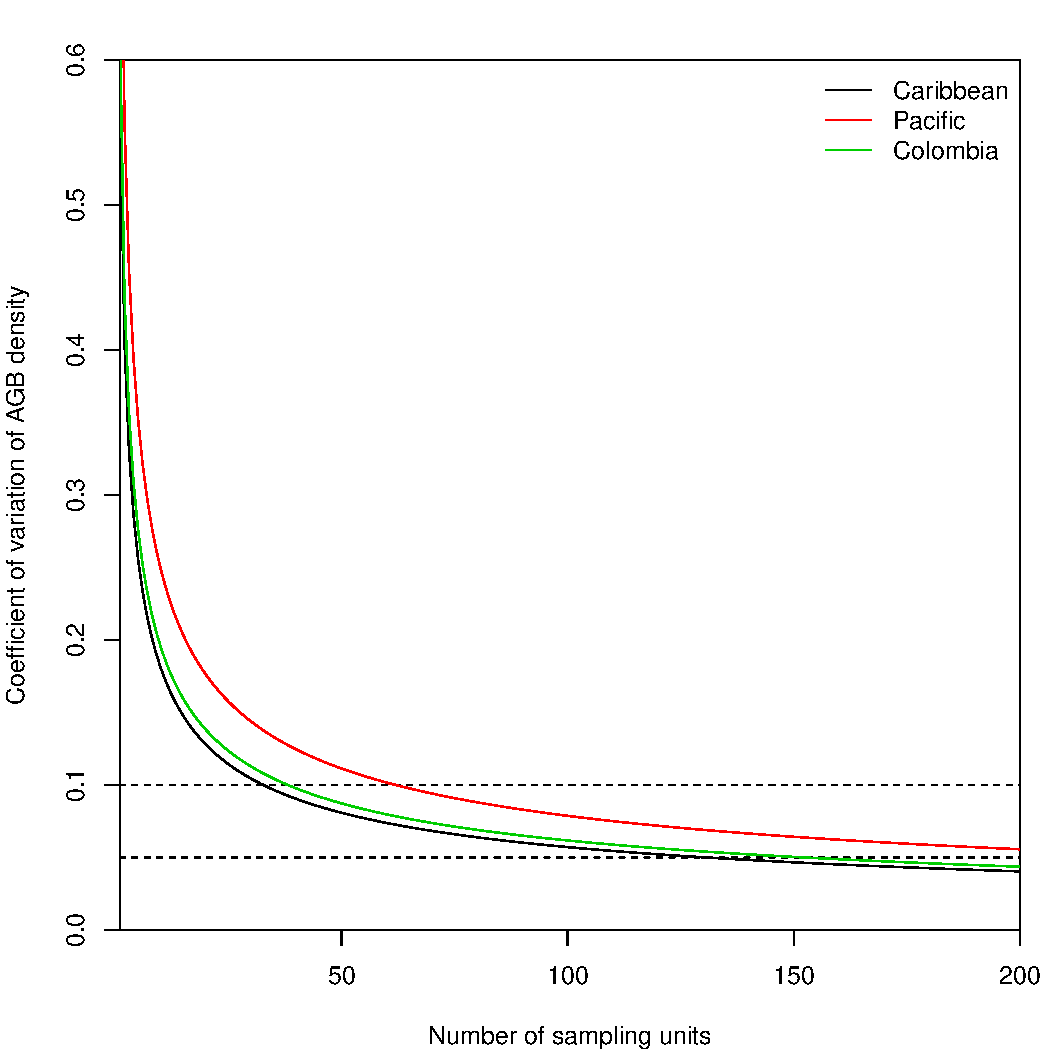
\includegraphics[%scale=0.4
%width=\textwidth
%]{Figures/AGBsamplingEffort.pdf} 
%\caption{
Figure 2. Number of necessary sampling units of AGB density required to reduce current uncertainties at 10\% and 5\% level for Caribbean, Pacific and total Colombian mangroves.%} \label{fig:samplingEffort}
%\end{figure}


\subsection{Predictive models}

We tested the ability of the models proposed by \citet{Twilley1992} and \citet{CONL:CONL12060}  in predicting our AGB density data. For both models, we found important overestimations of AGB density for the majority of the observations, although in some cases the models underestimated observed AGB density, particularly for values larger than 150-200 Mg ha$^{-1}$  (Figure 3 %\ref{fig:globalModels}).

%Comparison between AGB observed data and estimations made with the global models \citep{Twilley1992, CONL:CONL12060} shows that in both cases, global models underestimate the AGB for Colombian Mangroves(Figure 3). Due to this result, we decided to reparameterize those models using our data, looking for a best representation of the behaviour of our data with the new models.


%\begin{figure} 
%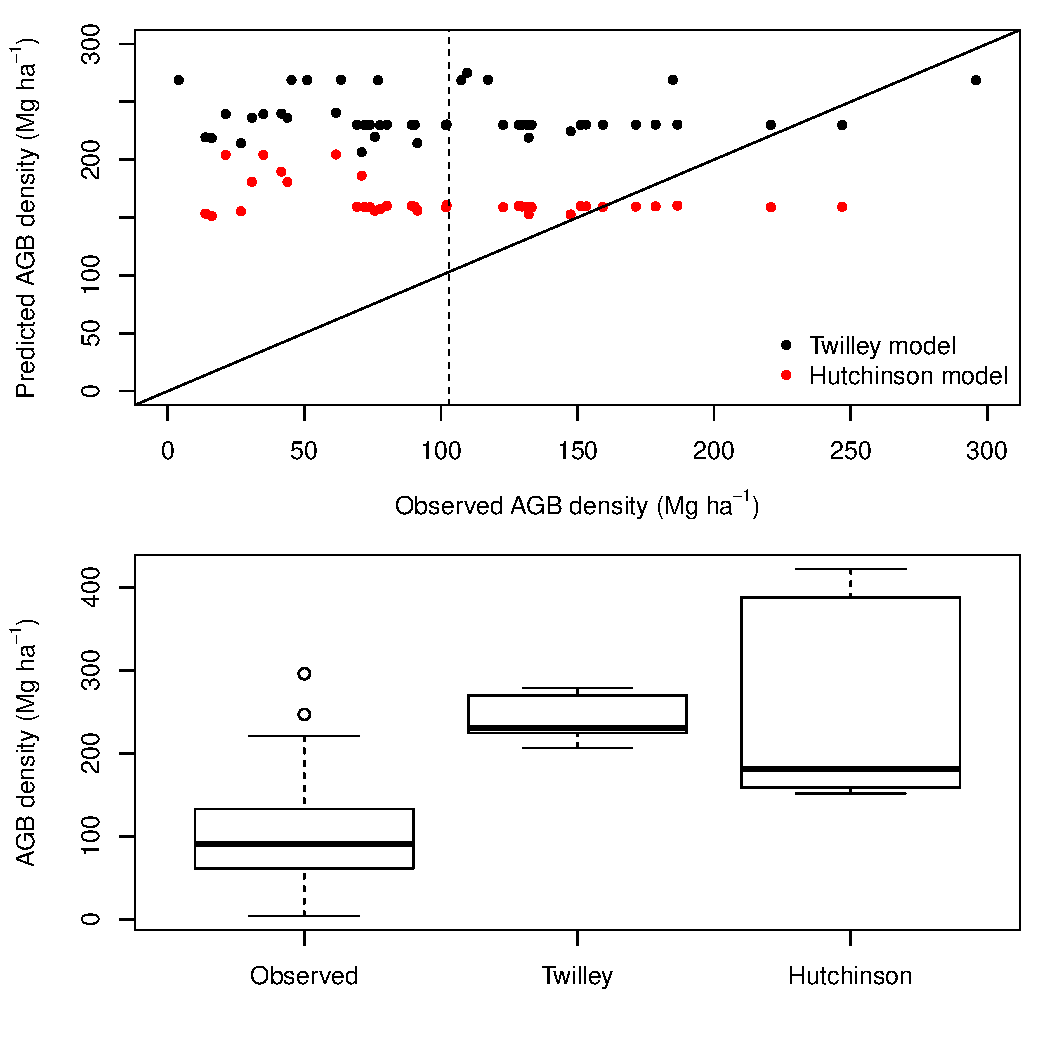
\includegraphics[%scale=0.4
%width=\textwidth
%]{Figures/Globalmodelsvs.pdf} 
%\caption{
Fiigure 3. Observed vs. predicted AGB density (Mg ha$^{-1}$). Predicted values: using global models \citep{Twilley1992, CONL:CONL12060} and observed data: current data available for mangrove areas in Colombia}% \label{fig:globalModels}
%\end{figure}


A  new parameterization of these models with our dataset provided a set of parameter values that can potentially help in estimating AGB density for our study area. However, the performance of the models as assessed by the R$_a^2$ statistic provided little confidence in these model structures in predicting accurately AGB density (Table \ref{tab:globalModels}).

% Requires the booktabs if the memoir class is not being used
\begin{table}[htbp]
   \centering
  
   \topcaption{Original models proposed by (1) \citet{Twilley1992} and (2) \citet{CONL:CONL12060} and the new parameterization obtained with our data. AGB represents  above ground biomass density (Mg/ha); Lat latitude (decimal degrees); BIO10 mean temperature of warmest quarter (\textcelsius); BIO11 mean temperature of coldest quarter (\textcelsius); BIO16 precipitation of the wettest quarter (mm); BIO17  precipitation of the driest quarter (mm) and R\textsubscript{a}\textsuperscript{2} adjusted coefficient of determination.} % requires the topcapt package
   \begin{tabular}{p{6.5cm}p{6.5cm}p{1.5cm}}  %Column formatting, @{} suppresses leading/trailing space
      \toprule
       Original model   & Reparameterized model & R\textsubscript{a}\textsuperscript{2}\\
      \midrule
       (1) AGB = -7.921$\cdot$Lat+298.5 & AGB = -1.266$\cdot$Lat+113.475   & -0.020\\
       (2) AGB = 0.295$\cdot$BIO10 + 0.658$\cdot$BIO11 + 0.023$\cdot$BIO16 + 0.195$\cdot$BIO17 - 120.3 & AGB = -0.2546$\cdot$BIO10 + 3.4824$\cdot$BIO11 + 0.2435$\cdot$BIO16 - 0.4056$\cdot$BIO17 - 875.7776 & 0.023\\ 
        \bottomrule
   \end{tabular}
   \label{tab:globalModels}
\end{table}

%\Jhoa {I don't want italics for BIO}

%According with R\textsubscript{a}\textsuperscript{2} criteria, those reparemeterized models do not explain the variability of our data. In the case of latitude-based model, the R\textsubscript{a}\textsuperscript{2} obtained in the reparameterized one (-0.01953) is much lower than the value associated with the original model and reported by \citet{Twilley1992} (0.75). Similarly, for the climate-based model developed by \citet{CONL:CONL12060}, reparemeterized model shows a R\textsubscript{a}\textsuperscript{2} value close to 0, much lower that R\textsubscript{a}\textsuperscript{2} associated with original model (0.267).

We tested 48 new model structures to predict AGB density with our data based on different combinations of the response functions in equations (1) to (5) applied to the bioclimatic variables of Table 1 as well as the values of latitude and EVI (see list of all models in appendix). From this group, six models were selected as candidate models due to their performance (Table \ref{tab:models}). 


 %Requires the booktabs if the memoir class is not being used
\begin{table}[htbp]s
   \centering
  \topcaption {Candidate statistical regression models selected based on their performance. AGB represents aboveground biomass (Mg/ha); log the natural logarithm; BIO9  the mean temperature of driest quarter (\textcelsius); BIO11 mean temperature of coldest quarter (\textcelsius); BIO16 the precipitation of the wettest quarter (mm); EVI is the enhanced vegetation index;  Lat latitude (decimal degrees); n is the number of observations; R\textsubscript{a}\textsuperscript{2} is the adjusted coefficient of determination; MSE is the mean squared error; F is the F-statistic; AICc Akaike's information criterion with a correction for finite sample sizes; AICcWt is the Akaike's weight}  % requires the topcapt package
   \begin{tabular}{p{7cm}p{0.5cm}p{1.0cm}p{1.0cm}p{1.0cm}p{1.0cm}p{1.0cm}}%Column formatting, @{} suppresses leading/trailing space
      \toprule
       Model  & n & R\textsubscript{a}\textsuperscript{2} & MSE & F & AICc & AICcWt\\
      \midrule
     $(1)\log{AGB}=-94.7756+21.9228\log{BIO9}-3.2190\log{BIO16}+0.8363\log{EVI}-1.1157\log{|Lat|}$&40&0.3586&0.489&6.452&94.12&0.01\\
     $(2)\log{AGB}=-18.7623+39.9688\log{BIO9}-3.0771\log{BIO16}+0.7138\log{EVI}-0.8834|Lat|-32.0563\log{BIO11}$ &40&0.353&0.493&5.256&96.26&0.00\\
     $(3)\log{AGB}=-68.661+21.023\log{BIO9}-5.397\log{BIO16}+1.842\log{EVI}-11.790\log{|Lat|}$&40&0.4507&0.419&9.00&87.92&0.19\\
     $(4)\log{AGB}=32.57-8256.48\frac{1}{BIO9}+572.76\frac{1}{BIO16}-6457.22\frac{1}{EVI}+21.75\frac{1}{|Lat|}$&40&0.4675&0.406&9.561&86.68&0.35\\
     $(5)\log{AGB}=-183.922+32.655\log{BIO9}+1.201\log{EVI}-2.282\log{|Lat|}$&40&0.3572&0.490&8.224&92.55&0.02\\
     $(6)\log{AGB}=36.25-8845.59\frac{1}{BIO9}-5303.93\frac{1}{EVI}+15.13\frac{1}{|Lat|}$&40&0.4507&0.419&11.67&86.27&0.43\\
      \bottomrule
  \end{tabular}
   \label{tab:models}
\end{table}


The selected models showed relatively similar values of R\textsubscript{a}\textsuperscript{2}. In all cases, the independent variables explained less than 47\% of total variability, but between the whole group of models,  they were between the best in terms of predictive power. Likewise, these six candidate models showed the lowest Mean Squared Error (MSE) values and higher values for the F-statistic. Additionally, independent variables were significant, Goldfeld-Quant test showed that candidate models do not present heterocedasticity problems, and according to the Durbin Watson test, there was not autocorrelation in the residuals. Cooks distance test did not evidence remote observations for any candidate model. 

Model 6 showed the lower value of AIC, indicating that this is the model with the best goodness of fit and higher simplicity of all compared models. Nevertheless, when AIC differences are very small, as in our case, the acceptance of one single model may lead to a false sense of confidence. In these cases, Akaike weights provide a straightforward interpretation as the probabilities of each model's being the best in the AIC sense. Using the AICcmodavg R package \citep{Mazerolle:2015aa}, we identified three model groups according with their weight: models (3), (4) and (6) were classified as models with ``substantial weight"; model (5) was classified as model with ``some weight''; while models (1) and (2) were classified  as models with ``little weight". The cumulative AIC weight of models (3), (4) and (6) represents 97\% of total, the remaining 3\% belonging to models (1) and (5). 

Even though the evidence ratio between models with ``substantial weight" indicates that model (6) is 1.23 times more likely than  the next-best model (4), we decided not to accept model (6) as the unique model recomended to predict carbon stocks in Colombian mangroves due to  the results from the AIC weights that indicate there is not enough evidence to chose only one model. Instead, we propose the biomass estimation through the use of weighted estimations of each of the three candidate models classified as models with ``substantial weight'' (models 6, 4 and 3).

Our candidate models included as predictive variables bioclimatology and a satellite-derived vegetation index, information that is easily accessible for all mangrove areas in Colombia. Nevertheless, models built with these variables did not show a very high predictive power. On the contrary, when a location variable such as ``site" or ``CEU'' was included in the models, the predictive power of all of them improved significantly, showing D\textsuperscript{2}\% around 86\%-87\% for all candidate models in the case of ``site'', and D\textsuperscript{2}\% around 46\%-65\%  in the case of ``CEU'' . The interaction site:CEU  did not contribute to explain of the variability in our data (Table \ref{tab:multilevel}).

%Requires the booktabs if the memoir class is not being used
\begin{table}[htbp]
   \centering
  \topcaption {Deviance analysis for candidate multilevel models through maximum likelihood estimation for AGB. When Site and CEU (Coastal Environmental Unit) are location variables;  AIC is the akaike information criterion; D\textsuperscript{2}\% is the Deviance}  % requires the topcapt package
   \begin{tabular}{p{2cm}p{4cm}p{2cm}p{2cm}p{2cm}p{2cm}}%Column formatting, @{} suppresses leading/trailing space
      \toprule
       Model  & Model modifications & AIC & Null deviance &Residual deviance & D\textsuperscript{2}\%\\
      \midrule
     (1) & Original model & 91.57& 29.75& 17.12 & 44.42\\
     (1) & Site & 60.01 & 29.75 & 3.86 & 87.02 \\
     (1) & CEU & 85.55 & 29.75 &12.06& 59.46 \\
     (1) & Site:CEU & 60.01 & 29.75 & 3.86 & 87.02 \\     
     (2) & Original model & 92.76 & 29.75 & 16.78 & 43.60 \\
     (2) & Site & 61.85 & 29.75 & 3.847 & 87.07\\
     (2) & CEU & 84.18 & 29.75 & 11.09 & 62.17 \\
     (2) & Site:CEU & 61.85 & 29.75 & 3.847 & 87.07 \\          
     (3) & Original model & 85.38 & 29.75 & 14.66 & 50.72 \\
     (3) & Site & 61.16 & 29.75 & 3.97 & 86.64 \\     
     (3) & CEU & 87.05& 29.75 & 12.52 & 57.92 \\     
     (3) & Site:CEU &61.16 & 29.75 & 3.97 & 86.64 \\          
     (4) & Original model & 84.13 & 29.75 & 14.21 & 52.24 \\
     (4) & Site & 62.65& 29.75 & 4.13 & 86.13\\
     (4) & CEU & 79.77 & 29.75 & 10.43 & 64.94 \\
     (4) & Site:CEU & 62.65& 29.75 & 4.13 & 86.13 \\
     (5) & Original model & 90.97 & 29.75 & 17.65 & 40.67 \\
     (5) & Site & 65.15 & 29.75 & 4.62 & 84.48 \\
     (5) & CEU & 94.85 & 29.75 & 15.99 & 46.25 \\
     (5) & Site:CEU & 65.15 & 29.75 & 4.62 & 84.48 \\
     (6) & Original model & 84.50 & 29.75 & 15.08 & 49.31 \\
     (6) & Site & 64.56 & 29.75 & 4.55 & 84.71 \\
     (6) & CEU & 88.05 & 29.75 & 13.49 & 54.66 \\
     (6) & Site:CEU &  64.56 & 29.75 & 4.55 & 84.71 \\
           \bottomrule
  \end{tabular}
   \label{tab:multilevel}
\end{table}


\subsection {AGB estimation using the predictive models}
Estimation of AGB density using the statistical models we developed, constrained their use to only sites that are within the range of values  of the independent variables considered in the analysis. Estimation for places located outside these ranges resulted in unrealistically high values of AGB density. For this reason, we only provide estimates for sites within the range of the input data used for the model development. 

Applying this restriction, the range of distribution of AGB density estimated from the selected predictive models, resulted in values between $\sim$40 and 200 Mg ha$^{-1}$. A map of the distribution of AGB density (Figure 4) shows the highest values for mangroves located in Cispatá Bay and Ci\'enaga Grande de Santa Marta (Caribbean coast), as well as San Juan river delta (Pacific coast). The average value of AGB density predicted using the statistical models was 75.62 $\pm$ 35.75 Mg ha$^{-1}$.

%\begin{figure} 
%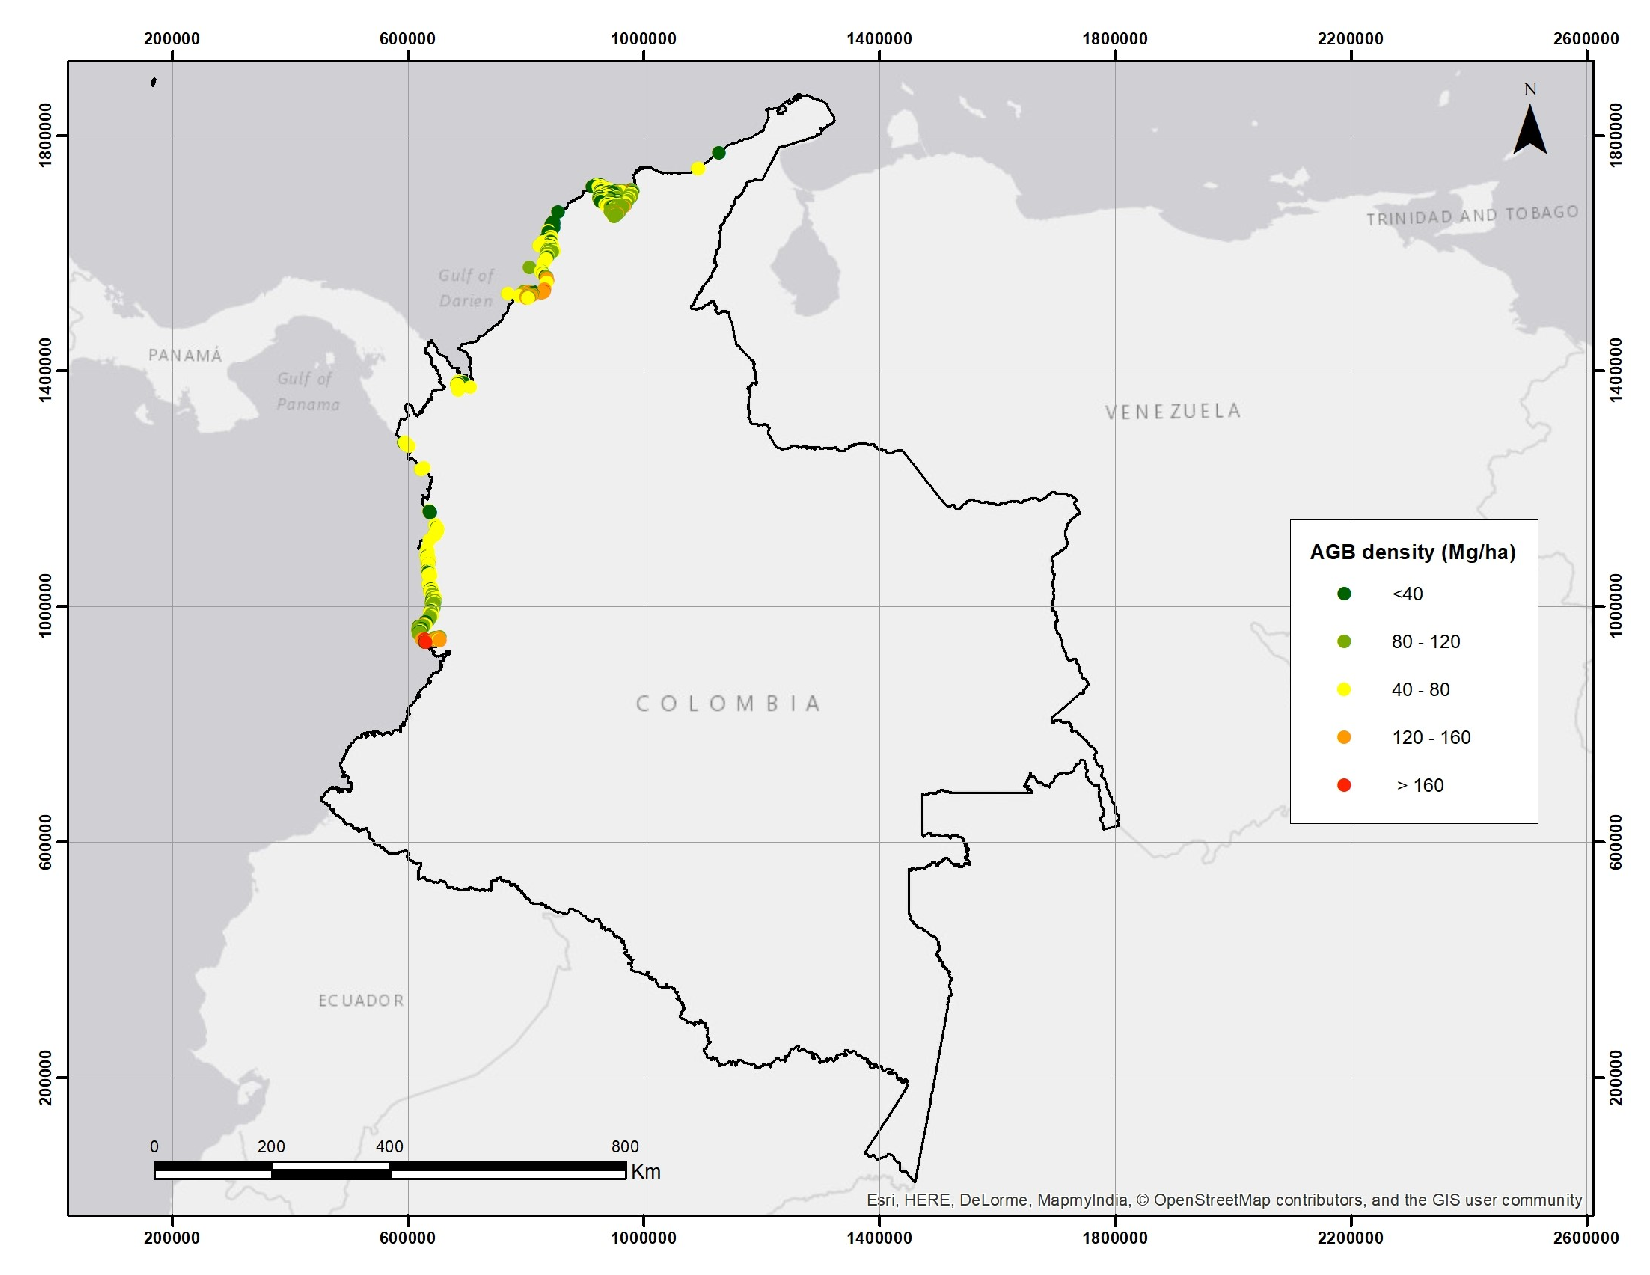
\includegraphics[%scale=0.4
%width=\textwidth
%]{Figures/AGBdensity_map_final.pdf} 
%\caption{
Figure 4. Map of predicted AGB density (Mg ha$^{-1}$) based on the candidate models classified as ``substantial weight models''%} %\label{fig:Predicted AGB density map}
%\end{figure}


\section{Discussion}
Using error propagation techniques, we were able to calculate the level of uncertainty that can be achieved with existing information for estimating aboveground C stocks for Colombian mangroves. This analysis showed that if Colombia wants to decrease the level of uncertainty in these estimations and include mangroves in its national GHG mitigation strategy, additional efforts are necessary to reduce uncertainty in both AGB density and mangrove area. We discuss here potential strategies to reduce these uncertainties and increase the quality of the estimates  to the Tier 3 level  as proposed by the IPCC \citep{IPCC2003, IPCC2006}. 


\subsection {Uncertainty and Tier 3 level estimates of national carbon stocks}

Discussion about uncertainties associated to total AGB carbon stocks for Colombian mangroves is addressed under the perspective of Tier approach. Carbon stock changes, emission and removals estimations have associated uncertainties, which in turn depend of the uncertainties of input data (AGB and mangrove area). In this regard, these uncertainties could be linked with some of the Tier levels according with the methods used for obtaining the data. Tier 1 uses data which can be obtained through national statistics, forest agencies, IPPC default values, survey and map agencies; Tier 2 uses country-defined national data sets; and, Tier 3 uses country-specific data \citep{IPCC2006}.

%Despite Tier levels are referred to changes in carbon stocks and areas, due to the estimation of total carbon stock for Colombian mangroves could be consider as start point for future analysis of GHG emissions/emissions reductions in terms of AFOLU category, the uncertainty level found for both AGB and mangrove area,  could be linked with some of the Tier levels according with the methods using for obtaining the data.

Currently, it is possible to estimate C stocks for Colombian mangroves at a Tier 2 level because there is available data on AGB density and mangrove area at a local level \citep{IPCC2003, IPCC2006}. However, we found poor quality in the data for mangrove area and had to rely on external sources for area estimation \citep[e.g.][]{Giri2011}; for this reason our best possible estimate of mangrove area is a combination of data of national sources and global and regional sources. 

%The decision about the use of global sources of mangrove area was made due to the official available data (provided by the Coastal and Marine National Research Institute (INVEMAR by its acronym in Spanish)) is a compilation of area estimations providing by different Governmental Environmental Agencies with jurisdiction in different mangrove areas along the country, which did not use the same scales and methodological approaches for the estimation and do not reference the uncertainty level associated to their estimations. These conditions lead to think that despite the uncertainty is not relate, it could be high and in this sense, for estimations at national level is better to use an average including other data published by external sources and estimate the associated uncertainty.

For REDD+ projects, it is appropriate to use Tier 2 data in the calculation of C stocks and avoided emissions \citep{Maniatis2010}, and our results suggest that it is currently possible to estimate C stocks in Colombian mangroves with a level of uncertainty that ranges between 18 to 39\% of the mean (Table \ref{tab:meansTotal}).
%Even problems associated with the use of different methodological approaches and not reported uncertainties for official mangrove areas estimation; both input data accomplish the suggestion of \citet{Maniatis2010} about the use of Tier 2 level in the context of REDD+. Additionally, this Tier is the same used in the framework of GHG emissions inventories of the country (SOURCE). 
Nevertheless, Colombia is in a transition to Tier 3 for the overall GHG national inventory, and to achieve this level the country is working on the firsts steps concerning the estimates of emissions factors for the AFOLU sector. The country is already working on a first phase of its national forest inventory \citep{IDEAM2015}, where mangroves should be treated as a separate ecosystem type for monitoring AGB density and area. 

%\Jhoa{I found in the Bianual Report 2014 that for AFOLU Tier is level 1. This data is different to Adri's info...maybe it changed?}

%Regarding our analysis approach, discrimination by coast not only give us a better idea about the differential potential of the mangroves areas as carbon sink along the country, but also provide us more precise information about the main source of uncertainty in carbon stock estimation and consequently it could allow decision makers to address in a best and more focal way the necessary efforts to reduce it. %The total uncertainty on a variable may be caused by both, random errors, which affect precision, and systematic errors (or biases), which affect accuracy \citep{Grassi2008}.

%For whole country uncertainties associated with mangrove area could be linked with the different methodological approaches used for its estimation, different scales of analysis and different quality of information. Indeed, at national level, data were not got under the same methodological approach  (official information is a compilation of independent estimations for every department with jurisdiction in mangrove areas) and estimations of this parameter do not relate the uncertainties. Different approaches could led to differences in definition and sampling design interpretation of samples \citep{IPCC2003}. Likewise, resolution of remote sensing and ground truth, error in census returns and positional error could be also sources of uncertainties in the estimation of area \citep{IPCC2003}.  In the specific case of Caribbean coast, uncertainties associated with area are specially relevant. This result could be highly influenced for the lower area estimation obtained using ArcGis approach with data got from \citet{Giri2011, Giri2011dataset} in comparison with other reported data. We included this estimation with the goal to capture the source of error associated overlapping layers (mangrove points and country border).

%Uncertainties are introduced at all stage of biomass estimation process \citep{Cohen2013968}, for this reason in the process to scale biomass estimation from plot or location level to coastal and national level, uncertainties are propagated and different errors linked with measurement, use of models, classification, data registration and calculation may occur during that process \citep{IPCC2006}. 
%AGB uncertainties are associated meanly to different scales of data derivation. Some of the data used comes from individual plots, while other correspond to extrapolations for wider areas. Likewise, the concentration of sampling and carbon estimation for some areas of the country is another important factor. While we found AGB information for four locations in the Caribbean coast %(La Guajira, Magdalena, C\'{o}rdoba and Antioquia departments) 
%for the Pacific coast, despite its bigger extension in terms of mangrove cover area, we only had access to AGB data in one location. %(Valle del Cauca department). 
%This situation don not necessary means that there is not additional information for this coast, but it shows that access to the information in the country is limited because of data are not sharing easily or there is not publications associated with some particular research efforts. 
%
%Not only more available data but also the good representation of the different types of mangroves  is a key reason for lower uncertainties found for AGB estimations in the Caribbean coast in comparison with Pacific coast. AGB data from the Caribbean comes from mangroves growing under different environmental conditions, representing the gradient of increased seasonality of precipitation and salinity from west to east \citep{Polania2015} which have a direct influence in the structure of the forest and the in the carbon allocation and dynamic. Meanwhile, the low representation of the different mangroves areas in the Pacific coast, which along the coast could show particular and contrasting estructural and floristic composition characteristics like answer to different physiographic conditions \citep{IIAP2009} could explain the higher uncertainties associated to AGB estimation. Nevertheless, this result does not mean that uncertainty associated to area is not relevant, it shows that besides an effort to improve precision and accuracy in area estimation is necessary to do an effort to reduce uncertainty in AGB estimation through a better representation of different types of mangroves ecosystems.

%Despite the main source of uncertainty for AGB carbon stock was identified for every coast, the decision about the efforts to reduce could be focused in the main source identified; or in both sources; or contrary to the suggested according with the results of this study, in the source that less uncertainty contribute for each coast in terms of total carbon stock. Making decisions is a complex process that not only take into account scientific and technical bases, but also political, logistic and economical reasons. In this sense our results involve suggestions from the scientific perspective but at the end, it is not the only way to address the topic. For this reason, despite for mangroves located in the Caribbean coast we identified uncertainties related with area as the most relevant, we also estimate the necessary extra effort to reduce total carbon stock uncertainties in terms of AGB accuracy and precision improvement, and in that way for both coasts as well as for the whole country we related additional sampling locations need to achieve uncertainties around 10\% level using a simulation process.


To achieve this Tier 3 level in mangrove ecosystems, it is important to increase the number of sampling units for AGB density and develop local assessments of mangrove area that are verified through field surveys. Our uncertainty analysis showed that more sampling units are required in both the Caribbean and the Pacific coasts to achieve a 10\% uncertainty of the mean AGB density. These sampling units should represent well the local level of variability within sites as suggested by the multilevel models (Table \ref{tab:multilevel}), and the estimation of areas should characterize this local level of variability as well if these models are to be used for prediction. There is already good evidence for a gradient of increased seasonality of precipitation and salinity from west to east in the Caribbean \citep{Polania2015}, and these ecological gradients must be captured both by the classification of areas in different groups and the AGB density that would correspond to each group. 

\subsection{Sensitivity of total uncertainty to uncertainty in mangrove area and AGB density}
Although there is not a level of uncertainty that is required or even recommended for monitoring C stocks in the AFOLU sector, we chose 10\% as a desired level to achieve. In this regard, the \citet{IPCC2003} mentions \emph{there is not a predetermined level of precision; uncertainty is assessed to help to prioritize efforts to improve accuracy in the future and guide decisions on methodological choice}. In this sense, a 10\% level of uncertainty as a goal can help in determining where to focus future monitoring efforts. Our sensitivity analysis showed that this 10\% level can only be achieved by reducing uncertainty in both mangrove area and AGB density, and keeping the current level of uncertainty in any of these two components is not an option to reduce overall uncertainty to 10\%. 

%For that reason our analysis in terms to achieve an uncertainty level in total C in ABG estimation of 10\% must be take as an example about the needed effort to get a desirable level. In the context of this example, despite for whole country mangroves  sensitivity analysis indicates there are more sampling units that needed to achieve 10\% of AGB density uncertainty, this requirement in terms of number of units is not enough if we do not have a good representation of AGB variability, as is the case of the Pacific mangroves were the low representation of ecosystems variability led to high uncertainties in terms of AGB density.

In the estimation of areas using remote sensing products, it is possible to achieve between 10 to 15\% uncertainty \citep{IPCC2003}, a level that is much lower than our current uncertainties in mangrove areas (16-37\%).  We believe this level of uncertainty can be achieved with much less effort than that required to reduce uncertainties for AGB density. With a 10\% uncertainty in area it is therefore necessary to reduce uncertainty in AGB density to 5\% (Table \ref{tab:sensCol}), which implies a large effort in terms of costs and logistics (to move from a level of 10\% to a level of 5\% almost three times more sampling units are needed). This is particularly difficult for mangroves in the Pacific coast where the current level of uncertainty in AGB density is 25\%. 

Based on these results, we recommend to develop a national assessment of mangrove areas using remote sensing products to achieve 10\% uncertainties and establish an additional set of monitoring plots in both coasts to reduce uncertainties to 5-10\%, with special focus on the Pacific where the mangroves are underrepresented. 

%Election of 10\% as minimum AGB density uncertainty level and remain consistent with 10\%-15\% uncertainty level which is possible to achieve for mangrove area estimation under remote sensing with ground based surveys approach \citep{IPCC2003}, leads to get uncertainty associated with total C AGB stock estimation in a rank between 14\% and 18\%.

%In general terms, to reduce uncertainties related with total AGB carbon stock estimation at coast level as well as at national level we propose the following ways in terms of area and AGB efforts, according with \citet{IPCC2003} recommendations:
%
Regarding the area estimation, the use the remote sensing data together with the ground based surveys approach  \citep{IPCC2003} has the advantage to be the most cost cost-efficient method of area measurement.Furthermore, in order to reduce the current uncertainties, it is important to check for a consistent relationship with the national area, to standardize definitions, to consult statistical agencies on likely uncertainties involved and to compare the results with international data sets. For the specific case of Colombia, the production of the official mangrove area statistics for the whole country must be led by an unique institution; the information used should derive from the same methodological approach, avoiding the current situation where different sources of information with unknowing uncertainties, different scales of analysis and use of remote sensing information from different years are used.

%
%\Jhoa{could be interesting to mention that IDEAM published a protocol for generating information on the distribution, extension and changes in forest cover of Colombia, from the Landsat image processing?}
%
Regarding the uncertainties related with the AGB estimation, homologation of approaches used for both field sampling and remote sensing tools are necessary. The implementation of a national mangrove inventory is probably the best way to ensure the use of the same approach and in this way reduce the current uncertainties. Nevertheless, in the case that mangrove national inventories are not contemplate, a general protocol to estimate biomass/carbon in mangroves should be proposed to ensure the use of a common methodological approach. The design of a national forest monitoring system for mangroves could also help to represent in a better way the variability of the carbon stocks in AGB due to differences between type of mangroves along both coasts. %Currently, due to the study of  mangroves are linked to particular initiatives, there are locations in the country (i.e. Ci\'{e}naga Grande de Santa Marta,  Cispat\'{a} bay and M\'{a}laga bay) better represented than other. 
%Furthermore, increasing the number of representative sample plots and measurements, further stratification of estimates on the basis of mangrove types are also important ways to reduce the uncertainties associated with the estimation of this parameter.
%
%At country level important advances in terms of AGB estimation propose have been achieved \citep{Phillips2014}. Nevertheless, the contribution of this study in terms of uncertainty estimation could be helpful in case that the country decide to improve the AGB estimation resolution from the current scale level (Holdridge life zone classification) to ecosystem level.

\subsection{Predictive models}
Predictive models of carbon stocks in mangrove ecosystem are an important tool for managers and decision makers because they provide a general idea about the potential as carbon sinks of different mangrove areas along the country, and help to prioritize efforts in terms of investment in research and development of pilot projects. They can also help to identify potential emissions due to land use change and design climate change mitigation projects. 

We found that previously published pantropical models for predicting carbon in mangroves fail at predicting our local observations of AGB density. Although these models are based on climatic variables known to predict well mangrove distributions worldwide, the models fail at predicting spatial heterogeneity at smaller scales, a limitation already recognized by model developers  \citep{CONL:CONL12060}.

%General world-wide models used do not explain the variability of our data. It could be due to the differences between scales. Despite climate variables and latitud used in those models are recognised for their high influence in AGB distribution in mangroves, the application of these global models along Colombian coast is not the best approach, because differences between the variables included could be not enough big and significant between locations to explain changes in the behaviour of AGB. In fact, \citet{CONL:CONL12060} highlighted like limitation, that fine-scale variation in forest structure is not captured in their model. 

Despite these limitations, we found that it is possible to develop accurate models using remote sensing information. In our case, models including EVI (enhanced vegetation index), Latitude and BIO9 (mean temperature of driest quarter) provided the best statistics in all cases. Some of the models also included the bioclimatic variable BIO16 (precipitation in the wettest quarter), consistent with previous studies that found good predictive power for these variables \citep{CONL:CONL12060, Herz1999, Anaya2009}. The fact that the chosen models include EVI, suggests that despite the possible introduction of noise given the use of marginal pixels, the EVI is still a sensitive variable for estimating biomass.

%Between the models developed with our own data (both reparameterized and new ones), models including EVI (enhanced vegetation index) and BIO9 (mean temperature of driest quarter) in all cases were the best. Some of them, also included the latitud and the bioclimatic variable BIO16 (precipitation in the wettest quarter). The relevance of extreme variables were also found by \citet{CONL:CONL12060} in their global climatic model. Distribution of temperature and precipitation are relevant in mangroves biogeography, density and forest height \citep{Herz1999}. On the other hand, EVI is a measure of greenness or cumulative greenness and has been used as a means to estimate biomass \citep{Anaya2009}.

We identified model structure as an additional source of uncertainty in estimating C stocks \citep[cf][]{IPCC2006}, and for this reason we do  not recommend one particular model but a set of three models that should be used together. We recommend to weigh the predictions from each of these three models according to the AIC and calculate prediction uncertainty accordingly. If additional information is available in terms of stratified areas for different sites, we recommend the use of multilevel models that account for spatial heterogeneity. 

%\citet{IPCC2006} indicated the existence of uncertainties associated with the structure of the models and highlighted the importance of identifying if the models structure are suitable before to use them for predictions. Five candidate models were identified and each one have an related weight according with the AIC results. In this sense, when we use a specific weight for each model we are associating uncertainty to the estimations derived from the use of those models. 
%
%Despite the predictive power of our candidate models were not bigger than 31\%, those models explain the national variation of AGB in a similar way that climated-based model \citep{CONL:CONL12060} explain the global variation. When location variable were include in the models they improved their predictive power significantly, explaining around three times more the variance. This result demonstrate the influence of the local variability in patterns of mangrove forest structure and function, changes in above-ground biomass and productivity \citep{Komiyama2008128, Krauss2008, Chen1999}. 
%
%Taking into account our climatic-based models do not have the capacity to captured this local variability, the estimations derived of them must be used carefully, more like in an exploratory mode. Candidate models can give a general idea about the capacity of Colombian mangroves like carbon sinks at national scale. For local estimations (i.e. at level of projects), we suggest the use of available AGB allometric models. %Our climatic models were developed with the goal to get national estimations through the use of variables of easy access. %The use of more specific information that could reflect in a better way the local variation is not possible because of the difference in the available data between locations. 
%
%To improve the predictive power of our candidate models and improve their capacity of explanation of the variability of our data, classification of mangroves under some category grouping different environmental and physiographic conditions that determine the differences in carbon stocks is necessary.  Under the perspective of this requirement, the identification of potential classification categories, likewise the identification of current information available as well as further studies is necessary.

 %Results of the mixed effect models demonstrated that the use of CEU like category to classify mangroves in the country is not useful. Despite this classification identify coastal units along the country with similar characteristics in terms of environmental variables and management, this division does not cover the high mangrove variability at local level, in this sense, it is possible to have different types of mangroves inside the same CEU category.
 
 \subsection {National AGB estimation using statistical models}
 Statistical models of AGB density based on easily available information such as EVI and climatic variables from WorldClim can be used to predict spatially explicit values of mangrove C stocks. However, care must be taken in not extrapolating these models beyond the range of values for which they were developed. 
Our results highlight the need to increase the number of AGB data from mangroves in a wider environmental spectrum to make more applicable and useful these statistical models. Nevertheless, our analysis shows the potential of using these models to predict local-scale variability in C stocks, and facilitate management and decision making at the national level. 

%Given the results, we recommend fitting the models using more AGB data. Limitation of data for this study settled in the difficulty accessing data. For knowing cases, AGB data exists but bureaucracy and/or the inexistent rugosity in the data treatment and custody makes impossible its access. A coordinate job between institutions working on this topic could help to reduce this kind of difficulties. Centralization of data in one institution could help not only to get together all data but also to standardize the methods for field and desk job and reduce uncertainties.

\section{Conclusions}
Two main sources of uncertainty contribute to the overall uncertainty in total carbon stocks in aboveground biomass for Colombian mangroves: uncertainty in mangrove area and uncertainty in AGB density. 
%Total carbon stock estimations for Colombian mangroves depend of the values of two parameters: area and AGB. Accuracy and precision associated with the estimation of these parameters incide directly in the uncertainty of carbon stocks estimated at coastal or country level.
Area is the main source of uncertainty for total carbon stocks in mangroves of the Caribbean coast, while AGB density is the main source of uncertainty for mangroves in the Pacific coast of Colombia. %Lower uncertainty associated AGB data for mangroves of the Caribbean coast in comparison with mangroves of the Pacific coast resides in a better representation of AGB in the Caribbean, while for Pacific mangroves despite to cover a bigger area with a high variability in terms of structure and floristic composition data are more scarce.

We predict a total carbon stock of 14.9 $\pm$ 2.7 Tg C in aboveground biomass for Colombian mangroves using a range of available information. 
To reduce the current levels of uncertainty in carbon stocks (from 18\% to 10\% of the mean) and achieve a Tier 3 level in accuracy as recommended by the IPCC, it is necessary to reduce uncertainty in mangrove area from 16 to 10\% and uncertainty in AGB density from 9 to 5\%. This could be achieved by increasing the amount of sampling units along both coasts for AGB inventories, with particular emphasis on the Pacific. Detailed estimations of mangrove areas with stratifications by mangrove type are also required to achieve this 10\% in overall uncertainty. 

%Reduction of current levels of uncertainty in total AGB carbon stocks, requires reduction of uncertainties in AGB and mangrove area estimation. Ways to reduce those uncertainties are directly related with homogeneity of approaches to get information related with these input data.
The reduction of uncertainty in the estimation of the total carbon in Colombia is a major technical challenge for the inclusion of mangrove ecosystem in national mitigation strategies. This reduction could be achieved focusing the efforts in reducing uncertainty associated to area estimation or AGB estimation. This study suggest the best way to achieve this reduction for each coast; nevertheless, selection of mangrove area or AGB to reduce uncertainty is a decision which implies other aspects related with capacities, logistic and financial resources.

%Global climate models does not capture the variability of Colombian mangroves at national scale. On the other hand, national models developed do not explain more that 31\% of the variability of our data. In this sense, multilevel models results suggest the relevance of local variability in the behaviour and distribution of AGB.
%
%There is not a unique model that could be explain the variability of our data. For that reason five candidate models are suggested for biomass estimations.  Candidate models can give a general idea about the capacity of Colombian mangroves like carbon sinks at national scale, nevertheless it is important to improve their predictive power and their capacity to explain the variability of our data including a location variable which allow grouping mangroves areas with similar environmental and physiographic conditions. %For local estimations (i.e. at level of projects), we suggest the use of AGB allometric models.
%
%Despite soil carbon is the main carbon compartment in mangrove ecosystems (in terms of carbon stocks), there is not enough data in Colombia to do an analysis as we presented with carbon associated with AGB. This situation demonstrate the necessity to increase the sampling in this compartment and in this way contribute with the improvement of the inventory of carbon stocks in this ecosystem in the country.

Models based on remote sensing information such as EVI and bioclimatic variables from WorldClim offer good opportunities to increase the level of detail and accuracy in predictions of mangrove carbon stocks, but these predictions need to account for model-structure uncertainty as well as local scale variability. Statistical models developed using these variables need to account for a wide range of environmental conditions, so predictions can be made for all possible combinations of environments in which mangroves occur. We propose here a set of models that account for a wide range of environmental conditions, but a new set of models with larger scope would have to be developed in the future addressing uncertainties in model structure, mangrove area, and AGB density estimation. 



\section*{Acknowledgements}
This study was conducted within the framework of the International Climate Protection Fellowships Programme of the Alexander von Humboldt Foundation funded by the German Federal Ministry for the Environment, Nature Conservation, Building and Nuclear Safety.
%The MOD13Q1 product was retrieved from the online Data Pool, courtesy of the NASA EOSDIS Land Processes Distributed Active Archive Center (LP DAAC), USGS/Earth Resources Observation and Science (EROS) Center, Sioux Falls, South Dakota, (https://lpdaac.usgs.gov/data\_access/data\_pool).
Special acknowledgement to GEF, UNDP, INVEMAR-MADS and CVS and other direct partners in the framework of the project COL-00075241, PIMS \# 3997 Design and Implementation of National Subsystem of Marine Protected Areas (SAMP by its Spanish acronym) in Colombia, to Fundaci\'on Natura Colombia in the framework of the MVC Colombia initiative and to the Research Center on Ecosystems and Global Change -Carbono \& Bosques for providing access to the database of AGB in Cispat\'a and M\'alaga bays.
%WORLDCLIM (BIOCLIMATIC VARIABLES)....WORLD CLIM NO PIDE SER INCLUIDO EN LOS AGRADECIMIENTOS..NI HUTCHINSON NI JARDINE LOS INCLUYEN, SOLO LOS CITAN EN EL TEXTO
%INDEPENDIENTE DE QUE EL MAX PLANCK SEA LA INSTITUCION DE AFILIACION DE LOS AUTORES TAMBIEN SE PONE EN LOS AGRADECIMIENTOS?
The Max Planck Institute for Biogeochemistry provided additional support for the development of this project. 


%Special acknowledgement for providing the access to the data base of AGB in Cispat\'{i}a and M\'{i}alaga bays to GEF, UNDP, INVEMAR-MADS and CVS and other direct partners in the framework of the project COL-00075241, PIMS \# 3997 Design and Implementation of National Subsystem of Marine Protected Areas (SAMP by its Spanish acronym) in Colombia, a nationally implemented project (NIM) in collaboration with the Bank of National Investment Projects. In the same way, to 'Fundaci\'{i}o Natura Colombia in the framework of the MVC Colombia initiative, co-supported by GEF through IBD and finally to the Administrative Department of Science, Technology and Innovation of Colombia (COLCIENCIAS by its Spanish acronym) through its Institutional Strengthening Program (2008-2011) which supported the participation of the Research Center in Ecosystems and Global Change -Carbono \& Bosques- in the establishment of permanent plots in these areas.


\section*{References}

\bibliography{Bibliography/Bibliography_Article_Mangroves}
%\bibliographystyle{apalike}


\end{document}  
